\section{Results}
\label{sec:results}

Approximately 130,000 speed datapoints or 26,000 seconds have been extracted from the dataset. The estimation performances of the trained models are presented in Figure \ref{resultsallF} and Table \ref{resultsallT}. The range of accuracy parameters were 0.14--0.36 m/s for \gls{mae} and 0.25--0.58 m/s for \gls{rmse}. The performance results of feature sets and methods are compared in the following sections.

\begin{table}[htbp] 
    \centering
    \caption{Accuracy of the models per feature sets. Window sizes are in timesteps. The accuracy results are shown in the form of \gls{mae} (\gls{rmse}) and are in meters per second.}% Add 'table' caption
\resizebox{\linewidth}{!}{%
       \begin{tabular}[H]{lcccccc}
    
    \toprule
    
    

 \multicolumn{1}{l}{\textbf{Feature set}} & \multicolumn{1}{l}{\textbf{Window}} &  \multicolumn{1}{c}{\textbf{\gls{svm}}} & \multicolumn{1}{c}{\textbf{Decision tree}} & \multicolumn{1}{c}{\textbf{Random forest}} & \multicolumn{1}{c}{\textbf{\gls{gbt}}} & \multicolumn{1}{c}{\textbf{\gls{gpr}}}\\
  
  \midrule
  
      \multicolumn{1}{l}{All} &\multicolumn{1}{c}{256} &  \multicolumn{1}{c}{\cellcolor{blue!40}0.16 (0.29)} & \multicolumn{1}{c}{\cellcolor{blue!25}0.18 (0.32)} & \multicolumn{1}{c}{\cellcolor{blue!50}0.14 (0.25)} & \multicolumn{1}{c}{\cellcolor{blue!13}0.20 (0.33)} & \multicolumn{1}{c}{\cellcolor{blue!40}0.16 (0.29)}\\
    
     & \multicolumn{1}{c}{128} & \multicolumn{1}{c}{\cellcolor{blue!25}0.18 (0.32)} &  \multicolumn{1}{c}{\cellcolor{blue!13}0.20 (0.35)} &  \multicolumn{1}{c}{\cellcolor{blue!35}0.17 (0.31)} &  \multicolumn{1}{c}{\cellcolor{red!10}0.23 (0.36)} &  \multicolumn{1}{c}{{\cellcolor{blue!25}0.18 (0.32)}} \\
    
    \multicolumn{1}{l}{Limbs} &\multicolumn{1}{c}{256} & \multicolumn{1}{c}{{\cellcolor{blue!25}0.18 (0.33)}} &  \multicolumn{1}{c}{\cellcolor{blue!13}0.20 (0.35)} &  \multicolumn{1}{c}{\cellcolor{blue!45}0.15 (0.27)} &  \multicolumn{1}{c}{\cellcolor{blue!10}0.22 (0.36)} &  \multicolumn{1}{c}{\cellcolor{blue!25}0.18 (0.32)}\\
    
        &\multicolumn{1}{c}{128}& \multicolumn{1}{c}{{\cellcolor{blue!18}0.19 (0.34)}} &  \multicolumn{1}{c}{\cellcolor{blue!10}0.21 (0.37)} &  \multicolumn{1}{c}{\cellcolor{blue!25}0.18 (0.33)} &  \multicolumn{1}{c}{\cellcolor{red!15}0.25 (0.39)} &  \multicolumn{1}{c}{\cellcolor{blue!13}0.20 (0.35)} \\
    
    \multicolumn{1}{l}{Sacrum/Withers} &\multicolumn{1}{c}{256} & \multicolumn{1}{c}{{\cellcolor{blue!18}0.19 (0.32)}} & \multicolumn{1}{c}{\cellcolor{blue!10}0.21 (0.36)} &  \multicolumn{1}{c}{\cellcolor{blue!40}0.16 (0.28)} & \multicolumn{1}{c}{\cellcolor{red!10}0.23 (0.37)} & \multicolumn{1}{c}{\cellcolor{blue!18}0.19 (0.33)}\\
    
    &\multicolumn{1}{c}{128}& \multicolumn{1}{c}{{\cellcolor{blue!10}0.21 (0.36)}} &  \multicolumn{1}{c}{\cellcolor{red!10}0.24 (0.39)} &  \multicolumn{1}{c}{\cellcolor{blue!10}0.21 (0.36)} &  \multicolumn{1}{c}{\cellcolor{red!15}0.25 (0.40)} &  \multicolumn{1}{c}{\cellcolor{blue!10}0.21 (0.36)} \\
    
    \multicolumn{1}{l}{Sacrum+Right front limb} &\multicolumn{1}{c}{256} & \multicolumn{1}{c}{{\cellcolor{blue!25}0.18 (0.30)}} &  \multicolumn{1}{c}{\cellcolor{blue!13}0.20 (0.34)} &  \multicolumn{1}{c}{\cellcolor{blue!45}0.15 (0.26)} &  \multicolumn{1}{c}{\cellcolor{blue!10}0.22 (0.35)} &  \multicolumn{1}{c}{\cellcolor{blue!35}0.17 (0.30)} \\

&\multicolumn{1}{c}{128}& \multicolumn{1}{c}{{\cellcolor{blue!13}0.20 (0.34)}} &  \multicolumn{1}{c}{\cellcolor{red!10}0.23 (0.37)} & \multicolumn{1}{c}{\cellcolor{blue!13}0.20 (0.34)}  & \multicolumn{1}{c}{\cellcolor{red!10}0.24 (0.39)}  & \multicolumn{1}{c}{\cellcolor{blue!10}0.21 (0.36)} \\

    \multicolumn{1}{l}{Sacrum}  &\multicolumn{1}{c}{256} & \multicolumn{1}{c}{\cellcolor{blue!10}0.21 (0.34)}  & \multicolumn{1}{c}{\cellcolor{red!10}0.23 (0.38)}  & \multicolumn{1}{c}{\cellcolor{blue!35}0.17 (0.29)}& \multicolumn{1}{c}{\cellcolor{red!10}0.24 (0.39)} & \multicolumn{1}{c}{{\cellcolor{blue!13}0.20 (0.34)}}\\
    
    &\multicolumn{1}{c}{128}& \multicolumn{1}{c}{\cellcolor{red!10}0.23 (0.38)} &  \multicolumn{1}{c}{\cellcolor{red!20}0.26 (0.42)} &  \multicolumn{1}{c}{\cellcolor{red!10}0.23 (0.38)} &  \multicolumn{1}{c}{\cellcolor{red!22}0.27 (0.42)} &  \multicolumn{1}{c}{{\cellcolor{red!10}0.23 (0.37)}} \\

    \multicolumn{1}{l}{Withers} &\multicolumn{1}{c}{256} & \multicolumn{1}{c}{\cellcolor{blue!10}0.22 (0.37)} &  \multicolumn{1}{c}{\cellcolor{red!10}0.24 (0.41)}  & \multicolumn{1}{c}{\cellcolor{blue!35}0.17 (0.31)}  & \multicolumn{1}{c}{\cellcolor{red!20}0.26 (0.42)}  & \multicolumn{1}{c}{{\cellcolor{blue!10}0.22 (0.36)}}\\
    
     &\multicolumn{1}{c}{128}& \multicolumn{1}{c}{\cellcolor{red!15}0.25 (0.42)} &  \multicolumn{1}{c}{\cellcolor{red!25}0.28 (0.46)} &  \multicolumn{1}{c}{\cellcolor{red!15}0.25 (0.42)} &  \multicolumn{1}{c}{\cellcolor{red!28}0.29 (0.46)} &  \multicolumn{1}{c}{{\cellcolor{red!15}0.25 (0.42)}}\\

    \multicolumn{1}{l}{Poll} &\multicolumn{1}{c}{256} & \multicolumn{1}{c}{\cellcolor{red!35}0.32 (0.53)} & \multicolumn{1}{c}{\cellcolor{red!40}0.35 (0.58)}  & \multicolumn{1}{c}{\cellcolor{red!35}0.28 (0.45)}  & \multicolumn{1}{c}{\cellcolor{red!45}0.36 (0.58)}  & \multicolumn{1}{c}{{\cellcolor{red!35}0.32 (0.52)}}\\
    
    &\multicolumn{1}{c}{128}& \multicolumn{1}{c}{\cellcolor{red!40}0.35 (0.57)} &  \multicolumn{1}{c}{\cellcolor{red!50}0.38 (0.61)} &  \multicolumn{1}{c}{\cellcolor{red!40}0.35 (0.57)} &  \multicolumn{1}{c}{\cellcolor{red!50}0.39 (0.61)} &  \multicolumn{1}{c}{{\cellcolor{red!50}0.38 (0.62)}} \\

    \multicolumn{1}{l}{Right front limb} &\multicolumn{1}{c}{256} & \multicolumn{1}{c}{\cellcolor{blue!13}0.20 (0.35)}  & \multicolumn{1}{c}{\cellcolor{red!10}0.23 (0.39)}  & \multicolumn{1}{c}{\cellcolor{blue!35}0.17 (0.31)}  & \multicolumn{1}{c}{\cellcolor{red!15}0.25 (0.40)}  & \multicolumn{1}{c}{{\cellcolor{blue!13}0.20 (0.35)}} \\ 
    
     &\multicolumn{1}{c}{128}& \multicolumn{1}{c}{\cellcolor{red!15}0.250.40} &  \multicolumn{1}{c}{\cellcolor{red!22}0.27 (0.43)} &  \multicolumn{1}{c}{\cellcolor{red!10}0.24 (0.40)} &  \multicolumn{1}{c}{\cellcolor{red!28}0.29 (0.45)} &  \multicolumn{1}{c}{{\cellcolor{red!10}0.24 (0.39)}} \\
 
    \multicolumn{1}{l}{Left front limb} &\multicolumn{1}{c}{256} & \multicolumn{1}{c}{\cellcolor{blue!10}0.21 (0.36)} &  \multicolumn{1}{c}{\cellcolor{red!10}0.23 (0.39)} &  \multicolumn{1}{c}{\cellcolor{blue!35}0.17 (0.31)} &  \multicolumn{1}{c}{\cellcolor{red!15}0.25 (0.40)} &  \multicolumn{1}{c}{{\cellcolor{blue!10}0.21 (0.35)}} \\
    
    &\multicolumn{1}{c}{128}& \multicolumn{1}{c}{\cellcolor{red!15}0.25 (0.40)} &  \multicolumn{1}{c}{\cellcolor{red!20}0.26 (0.43)} &  \multicolumn{1}{c}{\cellcolor{red!10}0.23 (0.39)} &  \multicolumn{1}{c}{\cellcolor{red!28}0.29 (0.45)} &  \multicolumn{1}{c}{{\cellcolor{red!10}0.23 (0.39)}} \\

    \multicolumn{1}{l}{Right hind limb} &\multicolumn{1}{c}{256} & \multicolumn{1}{c}{\cellcolor{blue!18}0.19 (0.33)} &  \multicolumn{1}{c}{\cellcolor{blue!10}0.21 (0.37)} & \multicolumn{1}{c}{\cellcolor{blue!40}0.16 (0.28)} & \multicolumn{1}{c}{\cellcolor{red!10}0.24 (0.38)} &  \multicolumn{1}{c}{{\cellcolor{blue!25}0.18 (0.33)}}\\ 
    
     &\multicolumn{1}{c}{128}& \multicolumn{1}{c}{\cellcolor{blue!10}0.22 (0.38)} &  \multicolumn{1}{c}{\cellcolor{red!20}0.26 (0.44)} &  \multicolumn{1}{c}{\cellcolor{blue!10}0.22 (0.39)} &  \multicolumn{1}{c}{\cellcolor{red!28}0.29 (0.46)} &  \multicolumn{1}{c}{{\cellcolor{blue!10}0.22 (0.39)}} \\ 

    \multicolumn{1}{l}{Left hind limb} &\multicolumn{1}{c}{256} & \multicolumn{1}{c}{{\cellcolor{blue!18}0.19 (0.33)}} &  \multicolumn{1}{c}{\cellcolor{blue!10}0.21 (0.36)} & \multicolumn{1}{c}{\cellcolor{blue!40}0.16 (0.28)}  & \multicolumn{1}{c}{\cellcolor{red!10}0.23 (0.38)}  & \multicolumn{1}{c}{\cellcolor{blue!25}0.18 (0.32)}\\
    
    &\multicolumn{1}{c}{128}& \multicolumn{1}{c}{{\cellcolor{blue!10}0.22 (0.38)}} &  \multicolumn{1}{c}{\cellcolor{red!15}0.25 (0.43)} &  \multicolumn{1}{c}{\cellcolor{blue!10}0.22 (0.38)} &  \multicolumn{1}{c}{\cellcolor{red!28}0.29 (0.46)} &  \multicolumn{1}{c}{\cellcolor{blue!10}0.21 (0.38)} \\
    
    \multicolumn{1}{l}{First 6 features of All^1} &\multicolumn{1}{c}{256} & \multicolumn{1}{c}{{\cellcolor{red!35}0.31 (0.51)}} &  \multicolumn{1}{c}{\cellcolor{red!50}0.39 (0.65)} & \multicolumn{1}{c}{\cellcolor{red!15}0.25 (0.43)}  & \multicolumn{1}{c}{\cellcolor{red!35}0.33 (0.56)}  & \multicolumn{1}{c}{\cellcolor{red!45}0.37 (0.59)}\\
    
    \multicolumn{1}{l}{First 6 features of two \gls{imu}^2} &\multicolumn{1}{c}{256} & \multicolumn{1}{c}{{\cellcolor{red!50}0.38 (0.65)}} &  \multicolumn{1}{c}{\cellcolor{red!55}0.42 (0.71)} & \multicolumn{1}{c}{\cellcolor{red!35}0.33 (0.56)}  & \multicolumn{1}{c}{\cellcolor{red!60}0.44 (0.76)}  & \multicolumn{1}{c}{\cellcolor{red!50}0.39 (0.64)}\\
    
    \multicolumn{1}{l}{First 6 features of one \gls{imu}^3} &\multicolumn{1}{c}{256} & \multicolumn{1}{c}{{\cellcolor{red!50}0.39 (0.65)}} &  \multicolumn{1}{c}{\cellcolor{red!60}0.44 (0.76)} & \multicolumn{1}{c}{\cellcolor{red!45}0.37 (0.60)}  & \multicolumn{1}{c}{\cellcolor{red!60}0.45 (0.78)}  & \multicolumn{1}{c}{\cellcolor{red!50}0.38 (0.64)}\\
    
       \bottomrule
       
       \multicolumn{7}{l}{\small $^1$ According to Table \ref{tablefeature}.}  \\
       
       \multicolumn{7}{l}{\small $^2$ Best performing six features from two \gls{imu}s feature sets (Table \ref{tablefeature}): Sacrum/Right front limb feature set.}\\
       
       \multicolumn{7}{l}{\small $^3$ Best performing six features from one \gls{imu} feature sets (Table \ref{tablefeature}): Right front limb feature set.}\\
       \end{tabular}}
    \label{resultsallT}
\end{table}

\subsection{\gls{gps} Validation Study}
A total of 450 speed values (range between 1.5 to 7.5 m/s) were collected using the \gls{gps} sensor. According to Table \ref{gps_1}, in the higher speeds, the error is higher as well. In contrast, the percentage of mean absolute error is lower in fast speed. 

\begin{table}[!htbp] 
    \centering
    \caption{\gls{gps} validation results}% Add 'table' caption
\resizebox{\linewidth}{!}{
       \begin{tabular}[H]{p{1cm}m{5cm}m{2cm}m{2cm}m{2cm}}
        \toprule
     & \multicolumn{1}{c}{\textbf{\gls{gps} speed} (\boldmath{\(\frac{m}{s}\)})}  & \multicolumn{1}{c}{\textbf{Video speed} (\boldmath{\(\frac{m}{s}\)})}  & &\\
    
    \cmidrule(lr){2-2} \cmidrule(lr){3-3}
    
     
    \multicolumn{1}{l}{\textbf{Speed}}& \multicolumn{1}{c}{Mean (Standard deviation)}  & \multicolumn{1}{c}{Mean (Standard deviation)} & \multicolumn{1}{c}{\textbf{\gls{mae}} (\boldmath{\(\frac{m}{s}\)})} & \multicolumn{1}{c}{\textbf{\gls{mape}(\%)}}\\
   
   
   
        \midrule
        
\multicolumn{1}{l}{Slow} & \multicolumn{1}{c}{1.71 (0.17)} &   \multicolumn{1}{c}{1.71 (0.16)} & \multicolumn{1}{c}{0.03} & \multicolumn{1}{c}{1.85\%}\\[0.4 em]
    
\multicolumn{1}{l}{Medium} & \multicolumn{1}{c}{4.35 (0.21)}  & \multicolumn{1}{c}{4.37 (0.23)} & \multicolumn{1}{c}{0.07} & \multicolumn{1}{c}{1.67\%}\\[0.4 em]
    
\multicolumn{1}{l}{Fast} & \multicolumn{1}{c}{7.49 (0.26)} &  \multicolumn{1}{c}{7.49 (0.26)} & \multicolumn{1}{c}{0.09} & \multicolumn{1}{c}{1.26\%}\\
    
        \bottomrule
    \end{tabular}}
    \label{gps_1}
\end{table}

\subsection{Comparison of Features, Algorithms, and Gaits}
%\subsection{Comparison of Selected Features}
According to Table \ref{tablefeature}, the first-ranked feature of upper body feature sets (sacrum, withers, poll, and Sacrum/Withers) was extracted from the z-axis of the accelerometer signal. The second-ranked feature was also from acceleration signals, which were derived from the x and z axes. For the limb feature sets, the z-axis of the angular velocity signal ranked the highest. Moreover, the second-ranked feature for both front limbs feature sets was obtained from the x-axis of the acceleration signal, while for both hind limbs and Limbs feature sets were selected from the z-axis of the gyroscope output. Furthermore, all the selected features of the limbs feature set were from the z-axis of angular velocity. 

\begin{table}[htb] 
    \centering
    \caption{The highest ranked (first to sixth) selected features using \gls{sffs} based on random forest method (256 timesteps windows). In this table, L: Left and R: Right.}% Add 'table' caption
\resizebox{\linewidth}{!}{%
       \begin{tabular}[H]{lcccccc}
    
    \toprule
    
    \multicolumn{1}{l}{\textbf{Feature set}} & \multicolumn{6}{c}{\textbf{Feature rank}}\\
    
 \cmidrule(lr){2-7}
    
    & \multicolumn{1}{c}{\textbf{First}} & \multicolumn{1}{c}{\textbf{Second}} & \multicolumn{1}{c}{\textbf{Third}} & \multicolumn{1}{c}{\textbf{Fourth}} & \multicolumn{1}{c}{\textbf{Fifth}}& \multicolumn{1}{c}{\textbf{Sixth}}\\
    
        \midrule
        
    \multicolumn{1}{l}{All}  & \multicolumn{1}{c}{max\_gyr$_z$} & \multicolumn{1}{c}{sd\_acc$_z$} & \multicolumn{1}{c}{mean\_gyro$_z$} & \multicolumn{1}{c}{p75\_gyr$_z$} & \multicolumn{1}{c}{{fft$_1$}\_acc$_x$} & \multicolumn{1}{c}{max\_acc$_x$} \\ [-0.1 em]
    
     & \multicolumn{1}{c}{(L hind)} & \multicolumn{1}{c}{(sacrum)} & \multicolumn{1}{c}{(sacrum)} & \multicolumn{1}{c}{(L front)} & \multicolumn{1}{c}{(withers)} & \multicolumn{1}{c}{(sacrum)} \\ [0.4 em]
    
    \multicolumn{1}{l}{Limbs} &  \multicolumn{1}{c}{max\_gyr$_z$} & \multicolumn{1}{c}{p75\_gyr$_z$} & \multicolumn{1}{c}{p25\_gyr$_z$} & \multicolumn{1}{c}{min\_gyr$_z$} & \multicolumn{1}{c}{p75\_gyr$_z$} & \multicolumn{1}{c}{p25\_gyr$_z$}\\ [-0.1 em]
    
      & \multicolumn{1}{c}{(L hind)} & \multicolumn{1}{c}{(L front)} & \multicolumn{1}{c}{(L hind)} & \multicolumn{1}{c}{(R hind)} & \multicolumn{1}{c}{(R hind)} & \multicolumn{1}{c}{(R front)}\\ [0.4 em]

        \multicolumn{1}{l}{Sacrum+} &  \multicolumn{1}{c}{sd\_acc$_z$} & \multicolumn{1}{c}{sd\_acc$_z$} & \multicolumn{1}{c}{ent\_gyr$_z$} & \multicolumn{1}{c}{p75\_acc$_x$} & \multicolumn{1}{c}{ent\_acc$_z$} & \multicolumn{1}{c}{skw\_acc$_z$}\\ [-0.1 em]
    
 \multicolumn{1}{l}{Withers} &     \multicolumn{1}{c}{(withers)} & \multicolumn{1}{c}{(sacrum)} & \multicolumn{1}{c}{(sacrum)} & \multicolumn{1}{c}{(withers)} & \multicolumn{1}{c}{(sacrum)} & \multicolumn{1}{c}{(sacrum)}\\ [0.4 em]
    
    \multicolumn{1}{l}{Sacrum+} &  \multicolumn{1}{c}{p25\_gyr$_z$} & \multicolumn{1}{c}{sd\_acc$_z$} & \multicolumn{1}{c}{max\_acc$_x$} & \multicolumn{1}{c}{mean\_acc$_x$} & \multicolumn{1}{c}{sd\_gyr$_y$} & \multicolumn{1}{c}{sd\_gyr$_z$}\\ [-0.1 em]
    
        \multicolumn{1}{l}{R front}& \multicolumn{1}{c}{(R front)} & \multicolumn{1}{c}{(sacrum)} & \multicolumn{1}{c}{(R front)} & \multicolumn{1}{c}{(sacrum)} & \multicolumn{1}{c}{(sacrum)} & \multicolumn{1}{c}{(R front)}\\ [0.4 em]
    
    \multicolumn{1}{l}{Sacrum} &   \multicolumn{1}{c}{min\_acc$_z$} & \multicolumn{1}{c}{sd\_acc$_z$} & \multicolumn{1}{c}{ent\_gyr$_z$} & \multicolumn{1}{c}{sd\_gyr$_x$} & \multicolumn{1}{c}{sd\_gyr$_y$} & \multicolumn{1}{c}{ent\_acc$_z$} \\ [0.4 em]
    
    \multicolumn{1}{l}{Withers} &  \multicolumn{1}{c}{sd\_acc$_z$} & \multicolumn{1}{c}{p75\_acc$_x$} & \multicolumn{1}{c}{sd\_acc$_x$} & \multicolumn{1}{c}{mean\_gyr$_z$} & \multicolumn{1}{c}{ent\_acc$_z$} & \multicolumn{1}{c}{sd\_gyr$_z$}\\ [0.4 em]
    
    \multicolumn{1}{l}{Poll} &  \multicolumn{1}{c}{{fft$_3$}\_acc$_z$} & \multicolumn{1}{c}{sd\_acc$_x$} & \multicolumn{1}{c}{sd\_gyr$_y$} & \multicolumn{1}{c}{ent\_acc$_z$} & \multicolumn{1}{c}{krt\_acc$_z$} & \multicolumn{1}{c}{ent\_acc$_x$}\\ [0.4 em]
    
     \multicolumn{1}{l}{R front} &  \multicolumn{1}{c}{p25\_gyr$_z$} & \multicolumn{1}{c}{max\_acc$_x$} & \multicolumn{1}{c}{sd\_gyr$_z$} & \multicolumn{1}{c}{mdn\_gyr$_z$} & \multicolumn{1}{c}{sd\_gyr$_y$} & \multicolumn{1}{c}{sd\_gyr$_x$}\\ [0.4 em]
    
     \multicolumn{1}{l}{L front} &  \multicolumn{1}{c}{p75\_gyr$_z$} & \multicolumn{1}{c}{max\_acc$_x$} & \multicolumn{1}{c}{sd\_gyr$_z$} & \multicolumn{1}{c}{sd\_acc$_y$} & \multicolumn{1}{c}{sd\_gyr$_y$} & \multicolumn{1}{c}{mdn\_gyr$_z$}\\ [0.4 em]
    
     \multicolumn{1}{l}{R hind} &  \multicolumn{1}{c}{min\_gyr$_z$} & \multicolumn{1}{c}{p75\_gyr$_z$} & \multicolumn{1}{c}{mdn\_acc$_x$} & \multicolumn{1}{c}{min\_acc$_x$} & \multicolumn{1}{c}{mean\_gyr$_x$} & \multicolumn{1}{c}{p75\_acc$_x$}\\ [0.4 em]
    
     \multicolumn{1}{l}{L hind} &  \multicolumn{1}{c}{max\_gyr$_z$} & \multicolumn{1}{c}{p25\_gyr$_z$} & \multicolumn{1}{c}{p75\_acc$_x$} & \multicolumn{1}{c}{mean\_gyr$_x$} & \multicolumn{1}{c}{min\_acc$_x$} & \multicolumn{1}{c}{p75\_acc$_y$}\\ [0.4 em]
    
        \bottomrule
    \label{tablefeature}
  \end{tabular}}
\end{table}

\begin{figure}[htbp]
\centering
\includegraphics[width=\linewidth]{chapters/Speed/figures/20201029.png}
\caption{Comparison of models performances using MAE(m/s) and \gls{rmse}(m/s).}
\label{resultsallF}
\end{figure}

%\subsection{Comparison of Feature Sets}
 It can be inferred from Figure \ref{resultsallF} and Table \ref{resultsallT} that All feature sets provided the best performance (\gls{rmse} = 0.25--0.33 m/s). In addition, the feature sets from both hind limbs IMU signals were labeled as the lowest \gls{rmse} and \gls{mae} among the individual IMU feature sets in estimating the speed (\gls{rmse} = 0.28 and \gls{mae} = 0.16 m/s). It should be noted that the accuracy of models except the model trained with poll features (\gls{rmse} = 0.45--0.58 m/s) were approximately as high as the model based on All feature set. Furthermore, splitting the data (200 Hz) in larger windows (256 timesteps) results in better performance of the model than smaller windows (128 timesteps) regardless of the regression method.

%\subsection{Comparison of machine learning algorithms}
Similar to the performance comparison of the feature sets, the differences between performances of models based on \gls{svm}, \gls{gpr}, and random forest methods were insignificant. Nonetheless, considering the small differences, the best machine learning method in terms of accuracy was the random forest method. Conversely, models based on decision tree and \gls{gbt} methods had the worst performance among the ML techniques used in this study.

%\subsection{Comparison of gait types}
As shown in Table \ref{resultsperrgait}, the \gls{rmse} and normalized \gls{rmse} increased and decreased respectively as the model estimated the faster gaits. The lowest \gls{rmse} (0.20 m/s) was obtained during walk, which was lower than the total \gls{rmse} (0.25 m/s). During pace, the model was indicated the lowest normalized \gls{rmse} (4.12\%) among other gaits.

\begin{table}[!htbp] 
    \centering
    \caption{Performance of model (based on ``All'' feature set, random forest method, and 256 timesteps windows) per gait type.}% Add 'table' caption
\resizebox{0.75\linewidth}{!}{
       \begin{tabular}[H]{lccc}
        \toprule
    
    \multicolumn{1}{l}{\textbf{Gait}} & \multicolumn{1}{c}{\textbf{Measured speed} (\boldmath{\(\frac{m}{s}\)})}  & \multicolumn{2}{c}{\textbf{Predicted Speed Error}}\\
    
    \cmidrule(lr){2-2} \cmidrule(lr){3-4}
    
     & \multicolumn{1}{c}{{Mean ($\pm$ Standard deviation)}}  &\multicolumn{1}{c}{\textbf{\gls{rmse}} (\boldmath{\(\frac{m}{s}\)})} & \multicolumn{1}{c}{\textbf{Normalized \gls{rmse}}} \\
     


        \midrule
        
\multicolumn{1}{l}{All} & \multicolumn{1}{c}{3.25 ($\pm 1.63$)} &   \multicolumn{1}{c}{0.25} & \multicolumn{1}{c}{7.69\%}\\[0.4 em]
    
\multicolumn{1}{l}{Walk} & \multicolumn{1}{c}{1.70 ($\pm 0.17$)}  & \multicolumn{1}{c}{0.20} & \multicolumn{1}{c}{11.76\%}\\[0.4 em]
    
\multicolumn{1}{l}{Trot} & \multicolumn{1}{c}{3.30 ($\pm 0.23$)} &  \multicolumn{1}{c}{0.31} & \multicolumn{1}{c}{10.03\%}\\[0.4 em]
    
\multicolumn{1}{l}{Tölt} & \multicolumn{1}{c}{3.90 ($\pm 0.23$)} & \multicolumn{1}{c}{0.28} & \multicolumn{1}{c}{7.18\%}\\  [0.4 em]

\multicolumn{1}{l}{Canter}& \multicolumn{1}{c}{4.95 ($\pm 0.43$)} & \multicolumn{1}{c}{0.34} & \multicolumn{1}{c}{6.87\%}\\ [0.4 em]
    
\multicolumn{1}{l}{Pace}& \multicolumn{1}{c}{7.52 ($\pm 1.43$)} & \multicolumn{1}{c}{0.31} & \multicolumn{1}{c}{4.12\%}\\ 


    
        \bottomrule
    \end{tabular}}
    \label{resultsperrgait}
\end{table}


\subsection{Model validation}
In total, 3600 speed values were generated from the datasets, where 2150 and 1450 speed values were from walk (1.63 ± 0.13 m/s) and trot (3.12 ± 0.18 m/s) respectively. The best performing method for speed estimation, random forest with 256 timestep window size, was selected for the validation study. The validation results were reported in Table \ref{imumocap_table}. According to the \gls{rmse} equation, the measured speed was derived from \gls{omc}, while the estimated speed was computed using the trained models.

\begin{table}[htb] 
    \centering
    \caption{Validation results of models based on random forest per feature sets compare to \gls{omc} derived speed data. Window sizes are 256 timesteps. The accuracy results are shown in the form of \gls{mae} (\gls{rmse}) and are in meters per second.}% Add 'table' caption
\resizebox{0.7\linewidth}{!}{
       \begin{tabular}[H]{p{2cm}m{2cm}m{2cm}m{2cm}}
        \toprule
    
    \multicolumn{1}{l}{\textbf{Feature set}} & \multicolumn{1}{c}{\textbf{Walk}}  & \multicolumn{1}{c}{\textbf{Trot}} & \multicolumn{1}{c}{\textbf{Walk+Trot}}\\
    
        \midrule
        
\multicolumn{1}{l}{All} & \multicolumn{1}{c}{0.15 (0.26)} &   \multicolumn{1}{c}{0.24 (0.41)} & \multicolumn{1}{c}{0.18 (0.33)}\\[0.4 em]
    
\multicolumn{1}{l}{Limbs} & \multicolumn{1}{c}{0.18 (0.31)} &   \multicolumn{1}{c}{0.30 (0.49)} & \multicolumn{1}{c}{0.21 (0.39)}\\[0.4 em]
    
\multicolumn{1}{l}{Sacrum/Withers}& \multicolumn{1}{c}{0.17 (0.28)} &   \multicolumn{1}{c}{0.24 (0.43)} & \multicolumn{1}{c}{0.20 (0.35)}\\[0.4 em]
    
\multicolumn{1}{l}{Sacrum/Right front limb}& \multicolumn{1}{c}{0.16 (0.28)} &   \multicolumn{1}{c}{0.25 (0.43)} & \multicolumn{1}{c}{0.19 (0.35)}\\  [0.4 em]

\multicolumn{1}{l}{Sacrum}& \multicolumn{1}{c}{0.18 (0.31)} &   \multicolumn{1}{c}{0.26 (0.44)} & \multicolumn{1}{c}{0.21 (0.39)}\\ [0.4 em]
    
\multicolumn{1}{l}{Withers}& \multicolumn{1}{c}{0.18 (0.33)} &   \multicolumn{1}{c}{0.28 (0.51)} & \multicolumn{1}{c}{0.21 (0.41)} \\ 

\multicolumn{1}{l}{Poll}& \multicolumn{1}{c}{0.32 (0.49)} &   \multicolumn{1}{c}{0.50 (0.76)} & \multicolumn{1}{c}{0.38 (0.61)}\\ 

\multicolumn{1}{l}{Right front limb}& \multicolumn{1}{c}{0.18 (0.33)} &   \multicolumn{1}{c}{0.27 (0.49)} & \multicolumn{1}{c}{0.21 (0.41)} \\ 

\multicolumn{1}{l}{Left front limb}& \multicolumn{1}{c}{0.18 (0.33)} &   \multicolumn{1}{c}{0.27 (0.49)} & \multicolumn{1}{c}{0.21 (0.41)} \\ 

\multicolumn{1}{l}{Right hind limb}& \multicolumn{1}{c}{0.17 (0.30)} &   \multicolumn{1}{c}{0.26 (0.46)} & \multicolumn{1}{c}{0.20 (0.37)} \\ 

\multicolumn{1}{l}{Left hind limb}& \multicolumn{1}{c}{0.17 (0.30)} &   \multicolumn{1}{c}{0.26 (0.46)} & \multicolumn{1}{c}{0.20 (0.37)} \\ 


    
        \bottomrule
    \end{tabular}}
    \label{imumocap_table}
\end{table}


\subsection{Resource usage}

The execution times of the models with 256 timestep windows were computed using the smartphone. The results presented in Table \ref{speedmodeltimes} are the time average of 1000 executions per model. decision tree and \gls{gbt} based models performed the fastest in all the four feature sets. Besides decision tree and \gls{gbt}, \gls{svm} and \gls{gpr} based models performed faster than random forest in a six features feature set, however, they performed slower as the number of features increased, in contrast to random forest.  

\begin{table}[htb] 
    \centering
    \caption{The smartphone execution time between models and feature sets. The time results are in milliseconds.}% Add 'table' caption
\resizebox{\linewidth}{!}{%
       \begin{tabular}[H]{p{3cm}m{2cm}m{2cm}m{2cm}m{2cm}m{2cm}m{2cm}}
    
    \toprule
    
    

 \multicolumn{1}{l}{\textbf{Feature set}} & \multicolumn{1}{l}{\textbf{Number of features}} &  \multicolumn{1}{c}{\textbf{\gls{svm}}} & \multicolumn{1}{c}{\textbf{Decision tree}} & \multicolumn{1}{c}{\textbf{Random forest}} & \multicolumn{1}{c}{\textbf{\gls{gbt}}} & \multicolumn{1}{c}{\textbf{\gls{gpr}}}\\
  
  \midrule
  
      \multicolumn{1}{l}{All} &\multicolumn{1}{c}{672} &  \multicolumn{1}{c}{777.81} & \multicolumn{1}{c}{< 0.01} & \multicolumn{1}{c}{44.13} & \multicolumn{1}{c}{0.10} & \multicolumn{1}{c}{1207.34}\\
    
     
    
    
    \multicolumn{1}{l}{Sacrum/Right front limb} &\multicolumn{1}{c}{192} & \multicolumn{1}{c}{279.99} &  \multicolumn{1}{c}{< 0.01} &  \multicolumn{1}{c}{33.71} &  \multicolumn{1}{c}{0.09} &  \multicolumn{1}{c}{431.18} \\

    \multicolumn{1}{l}{Right hind limb} &\multicolumn{1}{c}{96} & \multicolumn{1}{c}{172.45} &  \multicolumn{1}{c}{< 0.01} & \multicolumn{1}{c}{34.28} & \multicolumn{1}{c}{0.08} &  \multicolumn{1}{c}{240.14}\\ 
    
     
    \multicolumn{1}{l}{Top 6 features} &\multicolumn{1}{c}{6} & \multicolumn{1}{c}{22.15} &  \multicolumn{1}{c}{< 0.01} & \multicolumn{1}{c}{36.63}  & \multicolumn{1}{c}{0.08}  & \multicolumn{1}{c}{28.97}\\
    
       \bottomrule
    \end{tabular}}\\
      
    \label{speedmodeltimes}
\end{table}

The execution time of models versus their \gls{mae} is plotted in Figure \ref{timevsaccra}. The execution times between some models were very large, therefore, the logarithmic value of times were presented. The first, second, third, and fourth dot from left for each color is representative of the accuracy and execution time value of the related model on six features (from All feature set), Right front limb, Sacrum/Right front limb, and All IMUs feature sets. As presented earlier in Table \ref{resultsallT} and Figure \ref{resultsallF},  random forest yielded the best, and decision tree and \gls{gbt} yielded the worst performances. On the contrary, the execution times of \gls{gbt} and decision tree models were shorter than other models.

\begin{figure}[htbp]
\centering
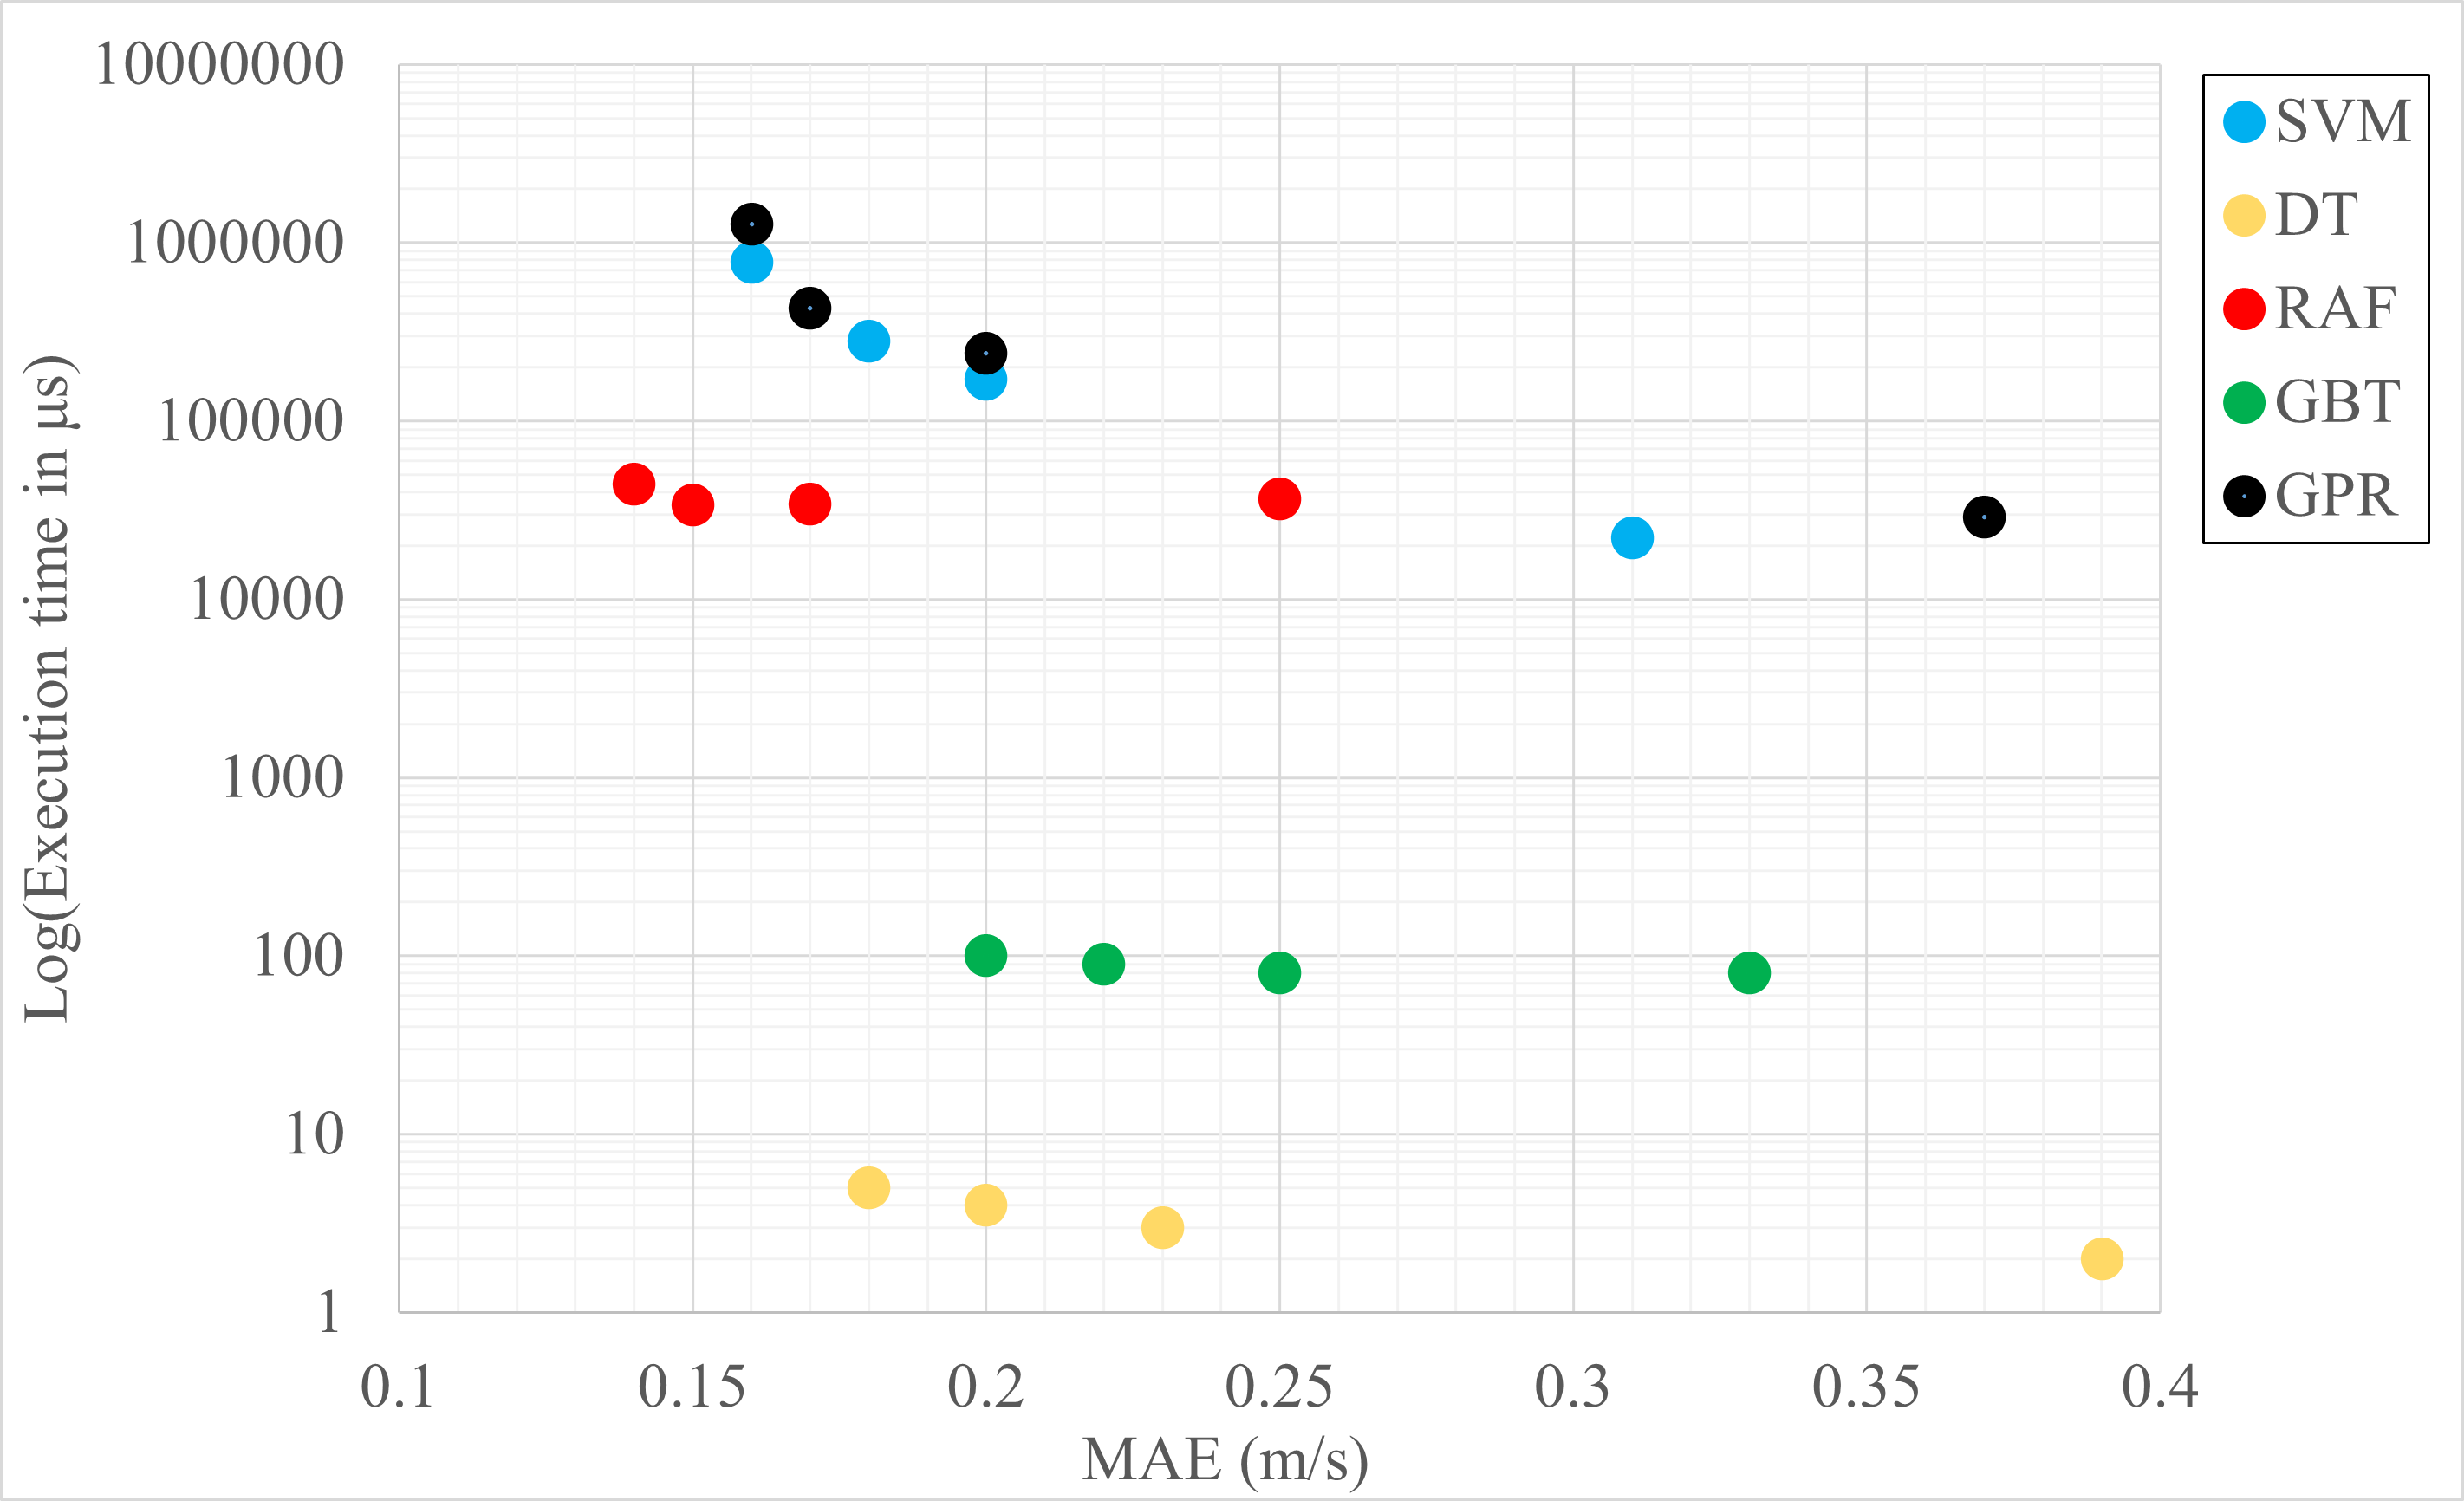
\includegraphics[width=.95\linewidth]{chapters/Speed/figures/Timevsaccuracy.png}
\caption{Comparison of models performances in terms of logarithm of execution times and accuracies (\gls{mae}). The first, second, third, and fourth dot from left for each color is representative of the accuracy and execution time value of the related model on six features (from All feature set), Right front limb, Sacrum/Right front limb, and All IMUs feature sets.}
\label{timevsaccra}
\end{figure}